\section{Техническое задание}
\subsection{Основание для разработки}

Основанием для разработки является задание на курсовую работу "<Разработка системы управления базами данных">.

\subsection{Цель и назначение разработки}

Основной задачей курсовой работы является разработка и тестирование собственной СУБД.

Посредством разработки и тестирование системы управления базами данных планируется улучшить понимание о внутренних процессах работы СУБД и разработать собственную систему управления базами данных.

Задачами данной разработки являются:
\begin{itemize}
\item реализация создания и удаления таблиц;
\item реализация чтения таблиц по определенным условиям;
\item реализация обновления таблицы;
\item реализация создания копий и сохранения таблиц в отдельный текстовый файл.
\end{itemize}

\subsection{Требования пользователя к интерфейсу СУБД}

Система управления базами данных должна включать в себя:
\begin{itemize}
    \item создание и удаление таблиц;
    \item работу с данными внутри таблиц;
    \item сохранение таблиц в отдельные файлы.
\end{itemize}

\subsection{Моделирование вариантов использования}

Для разрабатываемой системы управления базами данных была реализована модель, которая помогает понять использование СУБД.

На основании анализа предметной области в программе должны быть реализованы следующие прецеденты:
\begin{enumerate}
\item Добавление данных.
\item Обновление данных.
\item Удаление данных
\item Чтение и фильтрация данных.
\item Экспорт таблицы.
\end{enumerate}

На рисунке \ref{prec:image} изображена диаграмма прецедентов для СУБД.

\begin{figure}[ht]
	\center{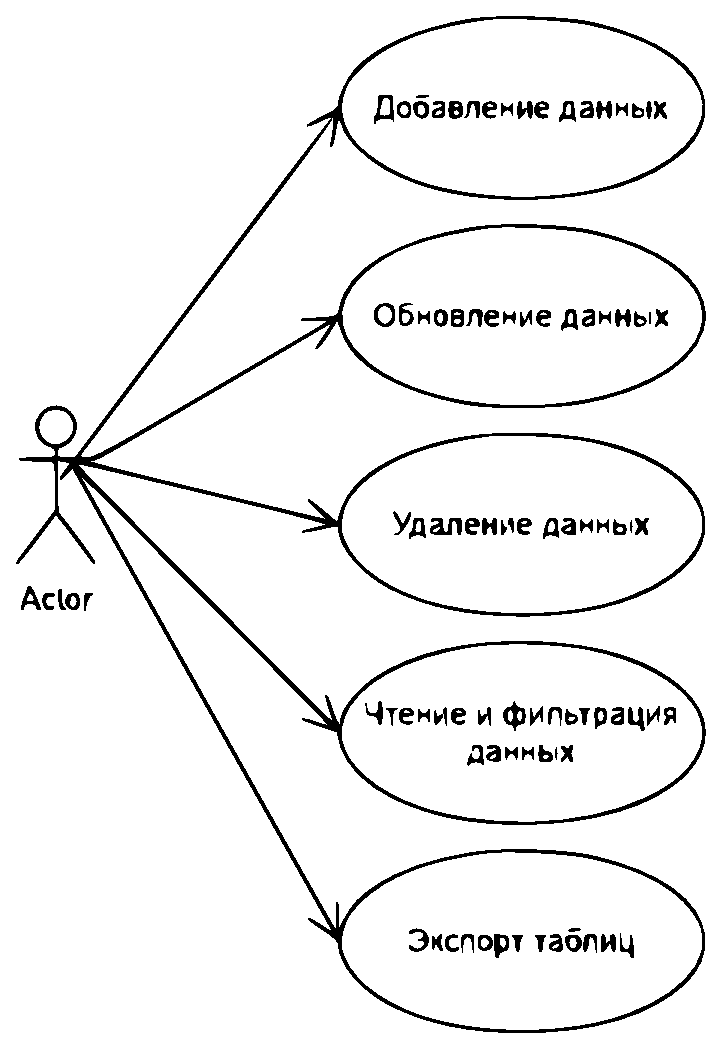
\includegraphics[width=1\linewidth]{prec}}
	\caption{Диаграмма прецедентов}
	\label{prec:image}
\end{figure}

\subsection{Требования к оформлению документации}

Разработка программной документации и программного изделия должна производиться согласно ГОСТ 19.102-77 и ГОСТ 34.601-90. Единая система программной документации.
